\UseRawInputEncoding
\documentclass{scrartcl}
\usepackage[utf8]{inputenc}
\usepackage[T1]{fontenc}
\usepackage[english]{babel}
\usepackage{lmodern}
\usepackage{color}
\usepackage[babel]{csquotes}
\usepackage{graphicx}
\usepackage{enumitem}
\usepackage{lscape}
\usepackage{booktabs}
\usepackage{hyperref}
\usepackage{float}
\usepackage{xcolor}
\usepackage[backend=biber]{biblatex}
\addbibresource{sources.bib}

\setcounter{secnumdepth}{0}

\title{Image classification with SVM}
\author{Andrea Portscher, Juan Pablo Stumpf, Philip Wille}

\begin{document}
\maketitle

\section{Introduction}
For this project we implemented an image classifier using three different feature extraction approaches: Scale-invariant feature transform (SIFT), Speeded up robust features (SURF) and Histogram of Gradients (HOG). First, we prepared an image dataset containing five different image classes, each comprising training and testing data. After extracting features using the above algorithms, we trained a Support-Vector Machine (SVM) and testetd, how well it was able to classify images.
\section{Approaches}
In the following section we will shortly explain the functionality of the feature extraction algorithms we applied to the dataset - namely SIFT, SURF and HOG.
In general, feature extraction algorithms work in three steps \cite{bay2006}:
\begin{enumerate}
  \item They select interest points at distinctive locations, such as corners.
  \item The neighbourhood of the interest points is represented by a feature vector.
  \item The descriptor vectors are matched between different images.
\end{enumerate}

\subsection{SIFT}


\subsection{SURF}
SURF is based on similar properties as SIFT but is - as the name already takes away - faster and more robust. In the detection phase, SURF approximates the Laplacian of Gaussian with a box filter, and a convolution with a box filter can can easily be calculated with the help of integral images, and can be parallelized for different scales.
Another improvement is the use of the sign of the Laplacian for underlying interest points in the matching phase. Since it is already calculated during the detection phase, it comes at no additional cost, but speeds up the process by only comparing features if they have the same type of contrast\footnote{https://docs.opencv.org/3.4/df/dd2/tutorial\_py\_surf\_intro.html}.

Unlike SIFT, the SURF algorithm is currently still patented and can therefore only be used by including the \texttt{opencv\_contrib} package\footnote{https://github.com/opencv/opencv\_contrib} and allowing non-free algorithms.

\subsection{HOG}

HOG stands for Histogram of Oriented Gradients and is a feature descriptor used in computer vision and image processing. Its purpose is to count the occurrence of gradient orientations in a given image. The first time HOG was described by Robert K. McConnell of Wayland Research Inc. in a patent application in 1986 without using the term. It has become more famous when Navneet Dalal and Bill Triggs \cite{Hog_article} presented their work on HOG descriptors in their 2005 published paper.

\subsubsection{Functionality of HOG}

HOG decomposes an image into small squared cells, computes a histogram of oriented gradients in each cell, normalizes the result using a block-wise pattern, and return a descriptor for each cell. Stacking the cells into a squared image region can be used as an image window descriptor for object detection, for example by means of an SVM.

\subsubsection{Preprocessing}

For using the HOG there is a recommended preparation step for the provided data. It's recommended to resize the image to a size of 64 by 128 pixels. This is because the implementation of the HOG used in the above mentioned paper of Navneet Dalal and Bill Triggs \cite[p. 4]{Hog_article}, combines 8 by 8 pixels to a cells, combines in turn 2 cells to a 16 by 16 pixel block and repeats this for the whole image.

\subsubsection{Implementation}

For implementing the HOG feature, we use the external library \href{https://scikit-image.org/}{scikit-image} for Python. The library itself offers a HOG\footnote{\href{https://scikit-image.org/docs/dev/auto_examples/features_detection/plot_hog.html}{Documentation of hog method}} method which executes the HOG feature on the provided image. We only modified the default values of the scikit-image implementation by changing following values:
\begin{itemize}
  \item The cells per block are set to 2 by 2 instead of 3 by 3. This has the effect, that the HOG feature only takes two cells for each block (16 pixels by 16 pixels each block) instead of three blocks (24 pixels by 24 pixels each block). With this change, we are more compliant with the paper of Navneet Dalal and Bill Triggs \cite[p. 4]{Hog_article}.
  \item Enabling square root transformation. This is not covered by the paper, but with this we achieved better results in comparison to the non enabled version.
\end{itemize}

\section{Implementation}
\subsection{Data}
The image data we used stems from the Caltech-256 Image Set\footnote{http://www.vision.caltech.edu/Image\_Datasets/Caltech256/, accessed on the 22nd of December 2020}, which consists of 256 sets of images of a certain class. We randomly selected 5 of these, namely: cactus, dice, raccoon, spaghetti and sushi. The preaparation of the image data was comprised of the following steps, which we implemented in the file \texttt{utils.py}:
\begin{itemize}
  \item All images were resized to the same size, converted to grayscale and normalized (which removes noise from the image).
  \item All images are associated with a label (their image class).
  \item The images are split into a training set (80\% of images per class) and a testing set (20\% of images).
\end{itemize}

\subsection{Pipeline}
We use a pipeline\footnote{https://scikit-learn.org/stable/modules/generated/sklearn.pipeline.Pipeline.html} which sequentially applies a list of transforms and a final estimator.
In our case the transformers are the application of the respective feature extractor and finally the SVM.
The SIFT and SURF transformers are initialized in the same manner: After the features have been extracted, they are clustered.
In this step we used the MiniBatchKMeans clustering algorithm\footnote{https://scikit-learn.org/stable/modules/generated/sklearn.cluster.MiniBatchKMeans.html}. We used the Elbow Method to approximate the ideal size for K.
This approach works by simply calculating and plotting the distortions as a function of the number of clusters. Then the "elbow" of the graph - meaning the point in which the number of distortions starts to decrease too slowly to justify the additional cost of an increase in the number of clusters. The resulting graph for SIFT can be seen on the following figure. On this base we chose the value 500.
\begin{center}
  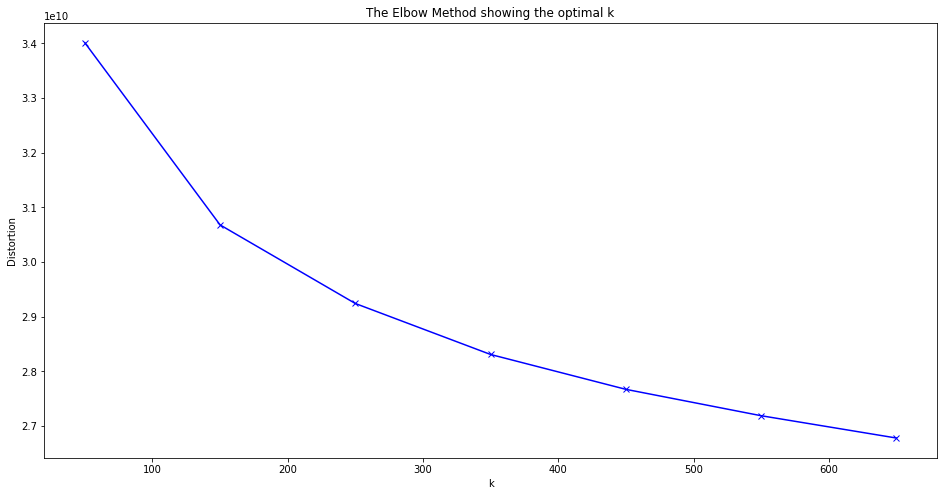
\includegraphics[scale=0.3]{img/kmeans-sift}
\end{center}
After having fitted the MiniBatchKMeans, the transformation begins and histograms are generated.
The next step in the pipeline is the training of the SVM. We chose the LinearSVC algorithm provided by the \texttt{sklearn} library\footnote{https://scikit-learn.org/stable/modules/generated/sklearn.svm.LinearSVC.html}.

\section{Discussion of Results}
In order to be able to evaluate our results we calculated metrics such as precision and recall and generated confusion matrices.
Furthermore, we used cross-validation. We checked the results for 2, 3, 4 and 5 image classes.
Naturally, all of the algorithms showed the best results with only 2 image classes and their reliability decreased with a rsing number of classes.

\printbibliography

\end{document}
